%%%%%%%%%%%%%%%%%%%%%%%%%%%%%%%%%%%%%%%%%%%%%%%%%%%%%%%%%%%%%%%%%%%%%%
%
% Dario Palminio
%
% LaTeX Template: Curriculum Vitae
%
% Source: http://www.howtotex.com/
% Feel free to distribute this template, but please keep the
% referal to HowToTeX.com.
% Date: July 2011
% 
%%%%%%%%%%%%%%%%%%%%%%%%%%%%%%%%%%%%%%%%%%%%%%%%%%%%%%%%%%%%%%%%%%%%%%
% How to use writeLaTeX: 
%
% You edit the source code here on the left, and the preview on the
% right shows you the result within a few seconds.
%
% Bookmark this page and share the URL with your co-authors. They can
% edit at the same time!
%
% You can upload figures, bibliographies, custom classes and
% styles using the files menu.
%
% If you're new to LaTeX, the wikibook is a great place to start:
% http://en.wikibooks.org/wiki/LaTeX
%
%%%%%%%%%%%%%%%%%%%%%%%%%%%%%%%%%%%%%%%%%%%%%%%%%%%%%%%%%%%%%%%%%%%%%%
\documentclass[paper=a4,fontsize=11pt]{scrartcl} % KOMA-article class
							
\usepackage[english]{babel}
\usepackage[utf8x]{inputenc}
\usepackage[protrusion=true,expansion=true]{microtype}
\usepackage{amsmath,amsfonts,amsthm}     % Math packages
\usepackage{graphicx}                    % Enable pdflatex
\usepackage[svgnames]{xcolor}            % Colors by their 'svgnames'
\usepackage{geometry}
	\textheight=700px                    % Saving trees ;-)
\usepackage{url}
\usepackage{wrapfig}

\frenchspacing              % Better looking spacings after periods
\pagestyle{empty}           % No pagenumbers/headers/footers

%%% Custom sectioning (sectsty package)
%%% ------------------------------------------------------------
\usepackage{sectsty}

\sectionfont{%			            % Change font of \section command
	\usefont{OT1}{phv}{b}{n}%		% bch-b-n: CharterBT-Bold font
	\sectionrule{0pt}{0pt}{-5pt}{3pt}}

%%% Macros
%%% ------------------------------------------------------------
\newlength{\spacebox}
\settowidth{\spacebox}{8888888888}			% Box to align text
\newcommand{\sepspace}{\vspace*{1em}}		% Vertical space macro

\newcommand{\MyName}[1]{ % Name
		\Huge \usefont{OT1}{phv}{b}{n} \hfill #1
		\par \normalsize \normalfont}
		
\newcommand{\MySlogan}[1]{ % Slogan (optional)
		\large \usefont{OT1}{phv}{m}{n}\hfill \textit{#1}
		\par \normalsize \normalfont}

\newcommand{\NewPart}[1]{\section*{\uppercase{#1}}}

\newcommand{\PersonalEntry}[2]{
		\noindent\hangindent=2em\hangafter=0 % Indentation
		\parbox{\spacebox}{        % Box to align text
		\textit{#1}}		       % Entry name (birth, address, etc.)
		\hspace{1.5em} #2 \par}    % Entry value

\newcommand{\CertificatesEntry}[2]{      % Same as \CertificatesEntry
		\noindent\hangindent=2em\hangafter=0 % Indentation
		\parbox{\spacebox}{        % Box to align text
		\textit{#1}}			   % Entry name (birth, address, etc.)
		\hspace{1.5em} #2 \par}    % Entry value	

\newcommand{\SkillsEntry}[2]{      % Same as \PersonalEntry
		\noindent\hangindent=2em\hangafter=0 % Indentation
		\parbox{\spacebox}{        % Box to align text
		\textit{#1}}			   % Entry name (birth, address, etc.)
		\hspace{1.5em} #2 \par}    % Entry value	
		
\newcommand{\EducationEntry}[4]{ % EducationEntry
		\noindent \textbf{#1} \hfill      % Study
		\colorbox{Black}{%
			\parbox{6em}{%
			\hfill\color{White}#2}} \par  % Duration
		\noindent \textit{#3} \par        % School
		\noindent\hangindent=2em\hangafter=0 \small #4 % Description
		\normalsize \par}

\newcommand{\WorkEntry}[4]{				  % WorkEntry Same as \EducationEntry
		\noindent \textbf{#1} \hfill      % Jobname
		\colorbox{Black}{\color{White}#2} \par  % Duration
		\noindent \textit{#3} \par              % Company
		\noindent\hangindent=2em\hangafter=0 \small #4 % Description
		\normalsize \par}

\newcommand{\CoursesEntry}[4]{				  % Same as \EducationEntry
		\noindent \textbf{#1} \hfill      % Jobname
		\colorbox{Black}{\color{White}#2} \par  % Duration
		\noindent \textit{#3} \par              % Company
		\noindent\hangindent=2em\hangafter=0 \small #4 % Description
		\normalsize \par}
		
		
%%% Begin Document
%%% ------------------------------------------------------------
\begin{document}
% you can upload a photo and include it here...
%\begin{wrapfigure}{l}{0.5\textwidth}
%	\vspace*{-2em}
%		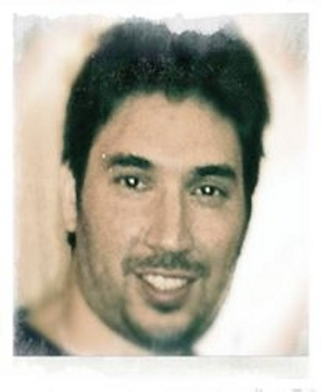
\includegraphics[width=0.15\textwidth]{photo}
%\end{wrapfigure}

%%% Photo
\begin{figure}
	\hfill
	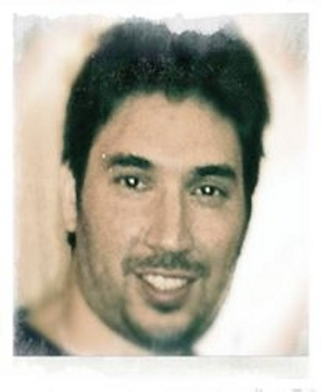
\includegraphics[width=0.2\textwidth]{photo}
	\vspace{-7cm}
\end{figure}

%%% Title
\MyName{Dario Palminio}
\MySlogan{Curriculum Vitae}

\sepspace

%%% Personal details
%%% ------------------------------------------------------------
\NewPart{Personal details}{}

\PersonalEntry{Birth}{January 6, 1977}
\PersonalEntry{Address}{5000 Cordoba, Argentina}
\PersonalEntry{Phone}{(000) 000-0000}
\PersonalEntry{Mail}{\url{dario.palminio@gmail.com}}
\PersonalEntry{Website}{\url{https://www.palminio.com}}
\PersonalEntry{linkedin}{\url{https://www.linkedin.com/in/palminio}}
\PersonalEntry{CScrumMaster}{\url{https://www.scrumalliance.org/community/profile/dpalminio}}

%%% Presentation
%%% ------------------------------------------------------------
\NewPart{Presentation}{
I'm a Systems Engineer graduated at the “National University of Southern Patagonia”, Argentina. So that's it, I am from Argentina. 
	As Systems Engineer I'm prepared to apply System Engineering, which is “an interdisciplinary approach and means to enable the realization of successful systems.”; And this generally includes the Software Engineering, that is “the application of a systematic, disciplined, quantifiable approach to the development, operation, and maintenance of software”. For this reason I have worked in both the software factories and in other areas.
}

%%% Education
%%% ------------------------------------------------------------
\NewPart{Education}{}

%2003 - Systems Engineer: School of Exact Sciences, UNPA-UACO National University. Graduated in 2003.
\EducationEntry{Systems Engineer}{2003}{UNPA-UACO National University}{Systems Engineer: School of Exact Sciences, UNPA-UACO National University. Graduated in 2003.}
\sepspace

%2000, Analyst: University Analyst Programmer: School of Engineering, UNPSJB University National. Graduated in 2000.
\EducationEntry{Analyst}{2000}{UNPSJB University National}{Analyst: University Analyst Programmer: School of Engineering, UNPSJB University National. Graduated in 2000.}
\sepspace

%1995, Electromechanical: Electromechanical technician: School ENET 1. Graduated in 1995.
\EducationEntry{Electromechanical}{1995}{School ENET 1}{Electromechanical: Electromechanical technician: School ENET 1. Graduated in 1995.}
\sepspace

%%% Work experience
%%% ------------------------------------------------------------
\NewPart{Work experience}{}

%2014-2015 Globant (globant.com) Software Engineer.
\WorkEntry{Globant/Latam}{2015-present}{ScrumMaster}
{Scrum Master in a context of Latam (LAN) airline at Globant Company.}
\sepspace

%2014-2015 Globant (globant.com) Software Engineer.
\WorkEntry{Globant}{2015}{Technical Leader, Focal point and Scrum Master}
{Technical Lead on Perl/Java Technologies in a context of LAN airline at Globant Company. The Perl Technologies used was Perl (POO with Moose, cgi, Test::Moore, Template Toolkit), MySQL, Linux, SVN, Git-Svn, CSS3, HTML5, Eclipse (RSE, EPIC), Review Board, Jenkins, etc. The Java Technologies used was SOAP, RESTful/RESTEasy, Spring, Maven, Javascript with front-end using MVC (Backbone.js). Project related to data collection from web site to send to Google Analytic.}
\sepspace

%2012-2014 IBA Entertainment limited as Software Engineer Freelancer.
\WorkEntry{IBA Entertainment limited}{2012-2014}{Software Engineer Freelancer}
{Software Engineer (as Contractor Freelancer) on Perl Technologies in a context of sportsbetting (Bet3000.com). Some technologies: Perl 5, EmbPerl Object, Object Perl, JSON, RESTful, Mojolicious, Perl DBI. Development in Bet3000 Project (www.bet3000.com) to International Betting Association.}
\sepspace

%2013-2014 Make IT Coop. As Associate, Secretary
\WorkEntry{Make IT Coop.}{2013-2014}{Associate, Secretary}{
Software Engineer}
\sepspace

%2008-2010 Motorola Mobility as Software Engineer.
\WorkEntry{Motorola Mobility}{2008-2010}{Software Engineer}
{Software Engineering on Java Technologies (J2EE in a context of telecommunications mobile devices) at Motorola Mobility of Argentina S.A.}
\sepspace

%2008-2010 Motorola S.C.A (Contractor Vates) as Software Engineer.
\WorkEntry{Motorola S.C.A (Contractor Vates)}{2008-2010}{Software Engineer}
{Java development (J2SE and J2EE in a context of telecommunications mobile devices)}
\sepspace

%2008 Vates (www.vates.com) as Systems Engineer.
\WorkEntry{Vates}{2008}{Systems Engineer}
{Java Developer in context of system business process management.}
\sepspace

%2007 Santex America S.A. (santexgroup.com) as Software Engineer: Java Developer.
\WorkEntry{Santex America S.A.}{2007}{Software Engineer, Java Developer}
{1) Java Developer in context of system business process management.}
\sepspace

%2007 AYI & Asociados (BADI S.R.L) as Software Engineer: Java Developer, Computer Consultant Java.
\WorkEntry{AYI and Asociados (BADI S.R.L)}{2007}{Software Engineer, Java Developer, Computer Consultant Java}
{1) Oracle Java Developer (J2EE) in context of credit card company (Tarjeta Naranja).
2) Instructor of "Oracle 9i: Build J2EE Applications" at InMotion, Santiago de Chile (Chile);
3) Instructor of "Oracle AS 10g: R3 Build J2EE Applications" at Oracle, Buenos Aires (Arg.).}
\sepspace

%2006 Informatic forensics – Tribunal third in Comodoro Rivadavia City: Informatic Forensics.
\WorkEntry{Tribunal third in Comodoro Rivadavia}{2006}{Informatic forensic}{
Tribunal third in Comodoro Rivadavia City: Forensic Engineering}
\sepspace

%2004-2006 24 months in Municipality of Comodoro Rivadavia city, Systems Engineer Juridical Informatics, Technical Leader.
\WorkEntry{Municipality of Comodoro Rivadavia}{2004-2006}{Systems Engineer Juridical Informatics, Technical Leader}
{Technical lead at Digesto Project (and VB Developer and PHP Developer) in context of legal area (Asesoría letrada) of a town hall (Municipality).}
\sepspace

%2004-2005 Teacher Mathematic Teacher, Software Teacher, Computation Teacher.
\WorkEntry{Teacher}{2004-2005}{Teacher Mathematic Teacher, Software Teacher, Computation Teacher}
{Profesor de Informática: 1- Computation Teacher I (Basic Informatic) - ISIS (Private Institute Third); 2- Computation Teacher II (Software Applications) - ISIS (Private Institute Third); 3- Computation Teacher III (Linux and Windows Net) - ISIS (Private Institute Third); Profesor de Software y Matemática (Mathematics and Software Teacher): 1- Course, Software Teacher: Adaptación al ambiente de trabajo en ENET 2 (technical school); 2- Course, Mathematic Teacher of 8-EGB  (two grades)- School 119 (C. R.); 3- Course, Mathematic Teacher of 9-EGB (two grades)- School 119 (C. R.).
}
\sepspace

%2000-2003 - DeSoft Development of Software
\WorkEntry{DeSoft}{2000-2003}{Developer, Technical Leader}{
Developer, Technical Leader}
\sepspace

%%% Certifications
%%% ------------------------------------------------------------
\NewPart{Certifications}{}

\CertificatesEntry{\large{\textbf{ScrumMaster}}}{}
\CertificatesEntry{}{
Certified ScrumMaster by SCRUM ALLIANCE.\newline
License: 000428099\newline
URL: \url{https://www.scrumalliance.org/community/profile/dpalminio}\sepspace
}
\sepspace


\CertificatesEntry{\large{\textbf{SDC}}}{}
\CertificatesEntry{}{
SCRUMstudy - Accreditation Body for Scrum and Agile.\newline
License: License 89793\newline
}
\sepspace

\CertificatesEntry{\large{\textbf{SMAC}}}{}
\CertificatesEntry{}{
Scrum Master Accredited Certification by International Scrum Institute.\newline
License: 59173583922442\newline
URL: \url{http://www.scrum-institute.org/International_Scrum_Institute_Certificate_Validation_Tool.php}
}
\sepspace

\CertificatesEntry{\large{\textbf{SPOAC}}}{}
\CertificatesEntry{}{
Scrum Product Owner Accredited Certification by International Scrum Institute.\newline
License: 92432962027378\newline
URL: \url{http://www.scrum-institute.org/International_Scrum_Institute_Certificate_Validation_Tool.php}
}
\sepspace

\CertificatesEntry{\large{\textbf{SC4JD}}}{}
\CertificatesEntry{}{
Scrum Certification for Java Developer by International Scrum Institute.\newline
License: 96122926946263\newline
URL: \url{http://www.scrum-institute.org/International_Scrum_Institute_Certificate_Validation_Tool.php}
}
\sepspace

%%% Courses
%%% ------------------------------------------------------------
\NewPart{Courses in management and organization}{}

\CoursesEntry{Course of Certified Scrum Master}{2015}{Kleer, Cba.-Arg.}{}
\CoursesEntry{Scrum Leader}{2015}{ValueInnova, Cba.-Arg.}{}
\CoursesEntry{Specialization in Project Management}{2010}{UTNFRBA, Bs.As.-Arg.}{}
\CoursesEntry{Project Management Career}{2008}{IAAP, PMI, Bs.As.-Arg.}{}
\CoursesEntry{Structuring Projects PM01.}{2007}{IAAP, Bs.As.-Arg.}{}
\CoursesEntry{Creation of Cooperatives.}{2012}{INAES, Cba.-Arg.}{}

\sepspace

%%% Skills
%%% ------------------------------------------------------------
\NewPart{Skills}{}

\SkillsEntry{\large{\textbf{Languages}}}{Spanish (mother tongue)}

\SkillsEntry{}{English (level 2)}

\sepspace

\sepspace

\SkillsEntry{\large{\textbf{Experience}}}{}
\SkillsEntry{}{
Regarding my professional career in general, I can say that I have around ten years of experience developing software, working widely not only in Software Engineering but also as part of Information Technology projects. I can tell you that I've worked for different international companies such as Santex America S.A., Motorola Mobility, IBA Entertainment limited and Globant. Also, I've had experience working remotely as a freelancer. Throughout this period, I participated in different software engineering roles. 
}

\sepspace

\SkillsEntry{\large{\textbf{Technologies}}}{}
\SkillsEntry{}{
Regarding my general experience on technologies, I've had wide exposure to a variety of software technologies and architectures, in a hands-on and directly-involved way. In other words I've used different types of technology and a lot of programming languages, such as Java, Perl, PHP, Python, C, etc.; but my favorite one is Java and all its related technologies, such as different framework to Java Enterprise Edition Platform (J2EE). This During the period that I work with Java I developed Web System using, among other things, the following technologies and frameworks: Hibernate, Maven, JavaScript, ExtJs, XML, JSF, Servlet, Spring, Resin, Tomcat, Oracle DB, MySQL DB, and PostgreSQL DB, JUnit, Mocks, SOA, etc.
}

\sepspace

\SkillsEntry{\large{\textbf{Domain}}}{}
\SkillsEntry{}{
	In my work history I've had experience in various domain problems. I made or worked in “airline” to LAN company, “Point Of Sale System” for a manufacturing company, “Machinery Maintenance System” for an oilfield services company, “Cemetery Management Systems” for a Municipal organization of a cemetery, “Legal Digest System” for a Town Council and Legislature, “Credit Card System” for a Credit Company, “Purchasing Management System” for a City Council,  “Business Process Management” System to Data Management Consultant Company, “System for Telecommunications and Internet Service Provider” for Telecommunications Companies and “Sportsbetting System” for an Online Betting Company.
}

%%% Top Technical Skills
%%% ------------------------------------------------------------
\NewPart{Top Technical Skills}{
About my Top technical skill I can mention Flexible Intelligence, Complex Problem Solving, Creative Thinking and Team player.
}

\sepspace

\SkillsEntry{\large{\textbf{Flexible Intelligence}}}{
I have a FAST LEARNING CURVE and ease to learn about any topic. This skill makes me ADAPTABLE and FLEXIBLE for perform in different work environments and different types of processes and technologies. In other words, I 'm always being open to change and to considerable variety in the workplace. I always think that I must to have the ability to adapt to change quickly and adjust work accordingly in a positive manner. There are three reasons why a software engineer should be a constant learner : a) A Systems Engineer must be able to understand different problem domains and each system is analyzed may involves new features and processes that are necessary to learn;  b) There is a low probability of participating in various projects and technology do not change; and c) The computer market behaves as the exponential growth of Moore's Law, this means that the technology and knowledge are improving at exponential rates. I take into consideration that the Systems Engineering should go hand in hand with Flexible Intelligence skill. In this regard, I have the aptitude and WILLINGNESS TO LEARN in a way beneficial to the business, the department and their own career. I'm able to effectively manage expectations and their own time, prioritizing according to communicated business requirements dynamically. 
}

\sepspace

\SkillsEntry{\large{\textbf{Complex Problem Solving}}}{
I think so that a good engineer has sharp problem solving skills. An engineer is frequently called upon solely to address problems, and they must be able to figure out where the problem stems from and quickly develop a solution. I am qualified to identifying complex problems in systems and reviewing related information to develop and evaluate options and implement solutions. Part of my activities as a developer have been to reduce code complexity and duplication, and to do structure and organizing software. To achieve this I have increased best practice utilization, reduced violations, avoided the carryover error, reduced defect rate and used proven development pattern. Also, from this perspective, I am trained to solve system problems using CRITICAL THINKING, that is scientific and logical thinking with Inquisitive mind. Also using aptitude for SYSTEMS THINKING and reasoning to identify the strengths and weaknesses of alternative solutions, conclusions or approaches to problems. Also, I have STRESS TOLERANCE and I've no problems with uncertainty and chaos. I consider that my profession relies on managing uncertainty and order the chaos. For this reason, I am familiar with uncertainty and THRIVE IN AMBIGUITY. In my working life I always have in my mind the following mantra (or slogan): “CHANGE THE COMPLEXITY TO MAKE IT SIMPLE AND ORDERED”. The “Order Emerges From Chaos” and for that we are Systems Engineers and Software Engineers, to make it possible.
}

\sepspace

\SkillsEntry{\large{\textbf{Creative Thinking}}}{
I have CREATIVE THINKING and alternative thinking to develop new ideas for and answers to work-related problems. At different times in my profession I have used creative thinking skills to contribute to a problem-solving software engineering team in a development project. I think so that a good engineer should be creative and can think of new and innovative ways to develop new systems and make existing things work more efficiently. Moreover, creating software requires creativity to make up solutions, designing new architectures, proposing new structures, implement high-level ideas and generate innovations. For all this creative thinking is necessary.
}

\sepspace

\SkillsEntry{\large{\textbf{Team Player}}}{
I like the team-oriented work environment.
}


%%% References
%%% ------------------------------------------------------------
\NewPart{References}{}

The following are some LinkedIn recommendations of my colleagues:

\sepspace

Senior Staff Software Engineer at Motorola Mobility:
«I had the chance to work closely with Dario during 2010 and 2011. Over that period of time he demonstrated high proficiency in J2EE, JavaScript, ExtJS programming languages, and technologies like TR69 and OMADM. Dario consistently completed his assignments, in particular the most technically challenging ones, which he was able to tackle thanks to one of his most important skills: creative thinking. I thank him for his contributions and extend my recommendation to whom it may concern.» 
May 1, 2012, Pablo Aghemo managed Dario indirectly at Motorola.

\sepspace

Staff Software Engineer at Motorola Mobility:
«I had the pleasure of working with Dario in several projects and in all that time he was consistently on schedule with his assignments. In those projects Dario always was a proactive professional. I think that he is a reliable person, very responsible and talented developer.»  
May 25, 2012, Diego Cohen worked directly with Dario at Motorola.

\sepspace

QA Engineer at Motorola Mobility:
«I would recommend Dario for whatever role he chooses, without any hesitation or concern for his success. His personality and versatility are remarkable skills that will take any project to success.»  
December 2, 2009, Franco Santi  worked directly with Dario at Motorola.

\sepspace

Software Engineer at Deviget LLC (2014):
«Dario is a highly skilled Systems professional. He has an extense background and experience on Software development, always focused and commited to achieve the expected results. I would recommend Dario to be part of any development team that need quick results as well as high quality products.»  
November 24, 2007, David Alderete was with another company when working with Dario at DeSoft.
Contact email:: david.ald@gmail.com; Contact celphone: +54-0351-3512445790

\sepspace

\end{document}
